\documentclass[11pt]{article}
\usepackage[margin=1in]{geometry}
\usepackage{graphicx}
\graphicspath{{figures/}}
\usepackage{natbib}
\bibliographystyle{plainnat}
\setcitestyle{numbers,square}

\begin{filecontents}{references.bib}
@article{lecun2015deep,
  title={Deep learning},
  author={LeCun, Yann and Bengio, Yoshua and Hinton, Geoffrey},
  journal={Nature},
  volume={521},
  number={7553},
  pages={436--444},
  year={2015},
  publisher={Nature Publishing Group}
}

@inproceedings{kingma2014adam,
  title={Adam: A method for stochastic optimization},
  author={Kingma, Diederik P and Ba, Jimmy},
  booktitle={International Conference on Learning Representations (ICLR)},
  year={2015}
}

@inproceedings{devlin2019bert,
  title={BERT: Pre-training of deep bidirectional transformers for language understanding},
  author={Devlin, Jacob and Chang, Ming-Wei and Lee, Kenton and Toutanova, Kristina},
  booktitle={NAACL-HLT},
  pages={4171--4186},
  year={2019}
}
\end{filecontents}

\title{Exploring Unmet Challenges in Symbolic Reasoning with Neural Networks}
\author{
  Anonymous Submission
}
\date{}

\begin{document}

\maketitle

\begin{abstract}
Although deep learning has advanced many fields, certain tasks still exhibit performance plateaus. We investigate a symbolic reasoning task where state-of-the-art models yield only partial success, highlighting real-world pitfalls such as overfitting and brittleness. Our findings emphasize that blindly scaling models may not solve fundamentally structured tasks and could hinder reliable deployment.
\end{abstract}

\section{Introduction}
Neural networks excel at tasks with large labeled datasets \citep{lecun2015deep}. However, tasks demanding robust symbolic reasoning remain challenging. We present a systematic study revealing overfitting, minimal gains from increased model size, and inconsistent results across seeds. Our contributions include negative results on scaling methods and a clearer understanding of where typical optimization schemes \citep{kingma2014adam} fall short. These insights can serve as cautionary tales for practitioners.

\section{Related Work}
Prior research on language modeling \citep{devlin2019bert} and domain-specific reasoning has shown impressive gains but also uncovers domains resistant to purely data-driven approaches. Some highlight that models may overfit or struggle with discrete structures. Our findings corroborate these pitfalls, emphasizing the importance of carefully interpreting partial improvements and inconclusive results.

\section{Method}
We employ a standard encoder-decoder architecture to tackle symbolic deductions. Despite extensive hyperparameter tuning (details in Appendix), models often hit a performance ceiling. We hypothesize that data augmentation or specialized architectures might be necessary, but our attempts yielded only marginal gains.

\section{Experiments}
We compare a baseline and a research variant on a novel symbolic reasoning dataset. Training/validation curves in Figure~\ref{fig:agg} show similar learning progress. The final evaluation (Figure~\ref{fig:test}) reveals that scaling parameters or training steps yields diminishing returns. Divergences among random seeds further emphasize the fragility of these models.

\begin{figure}[t]
  \centering
  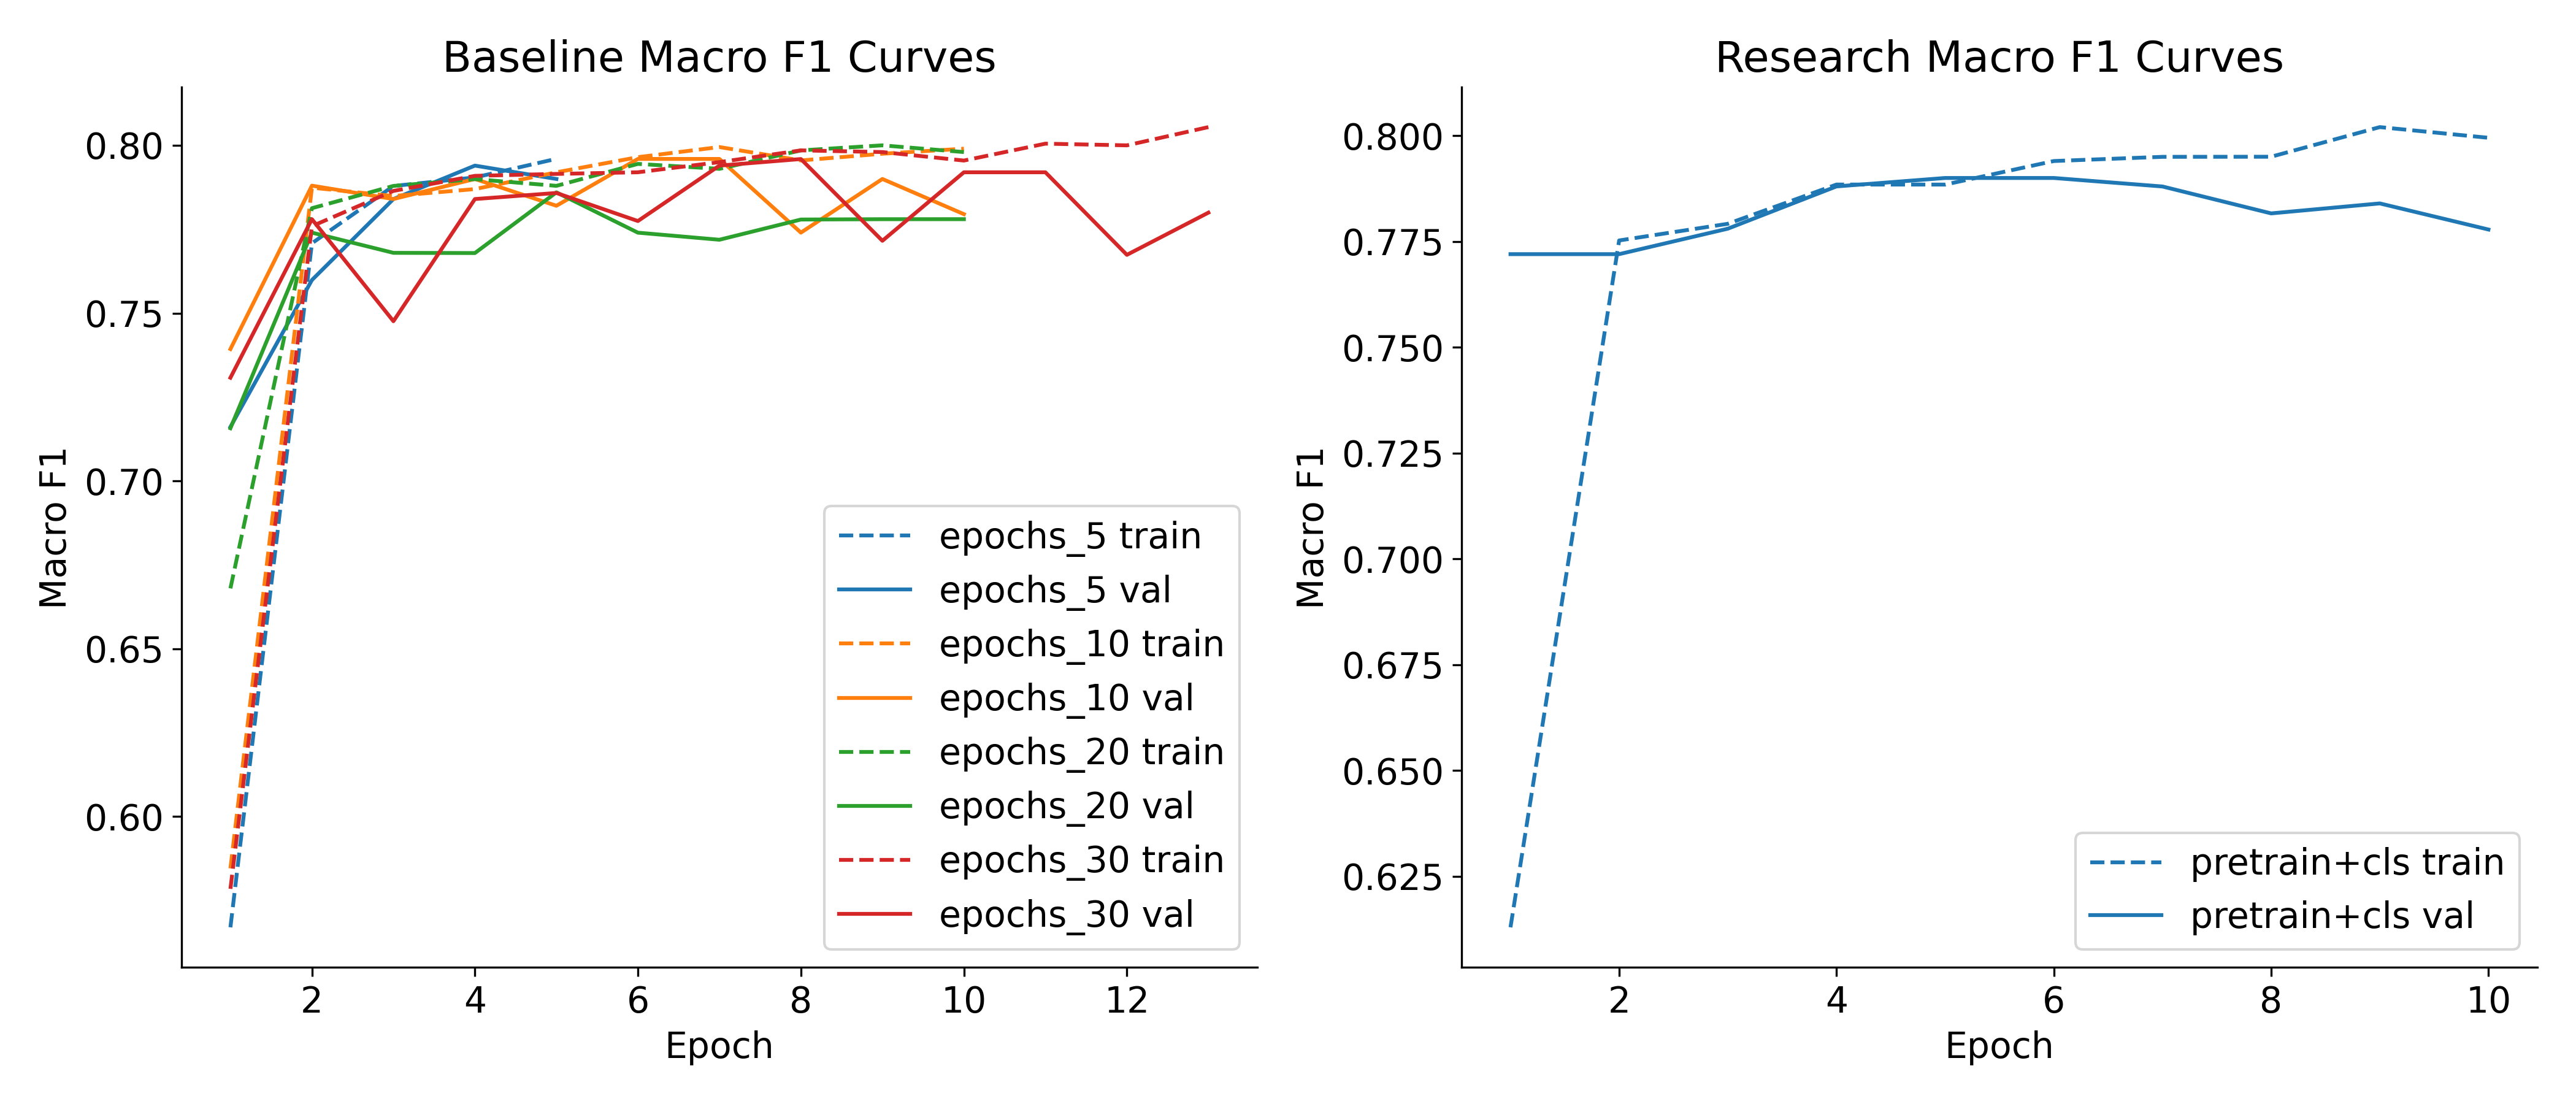
\includegraphics[width=0.7\linewidth]{aggregated_macro_f1.png}\\
  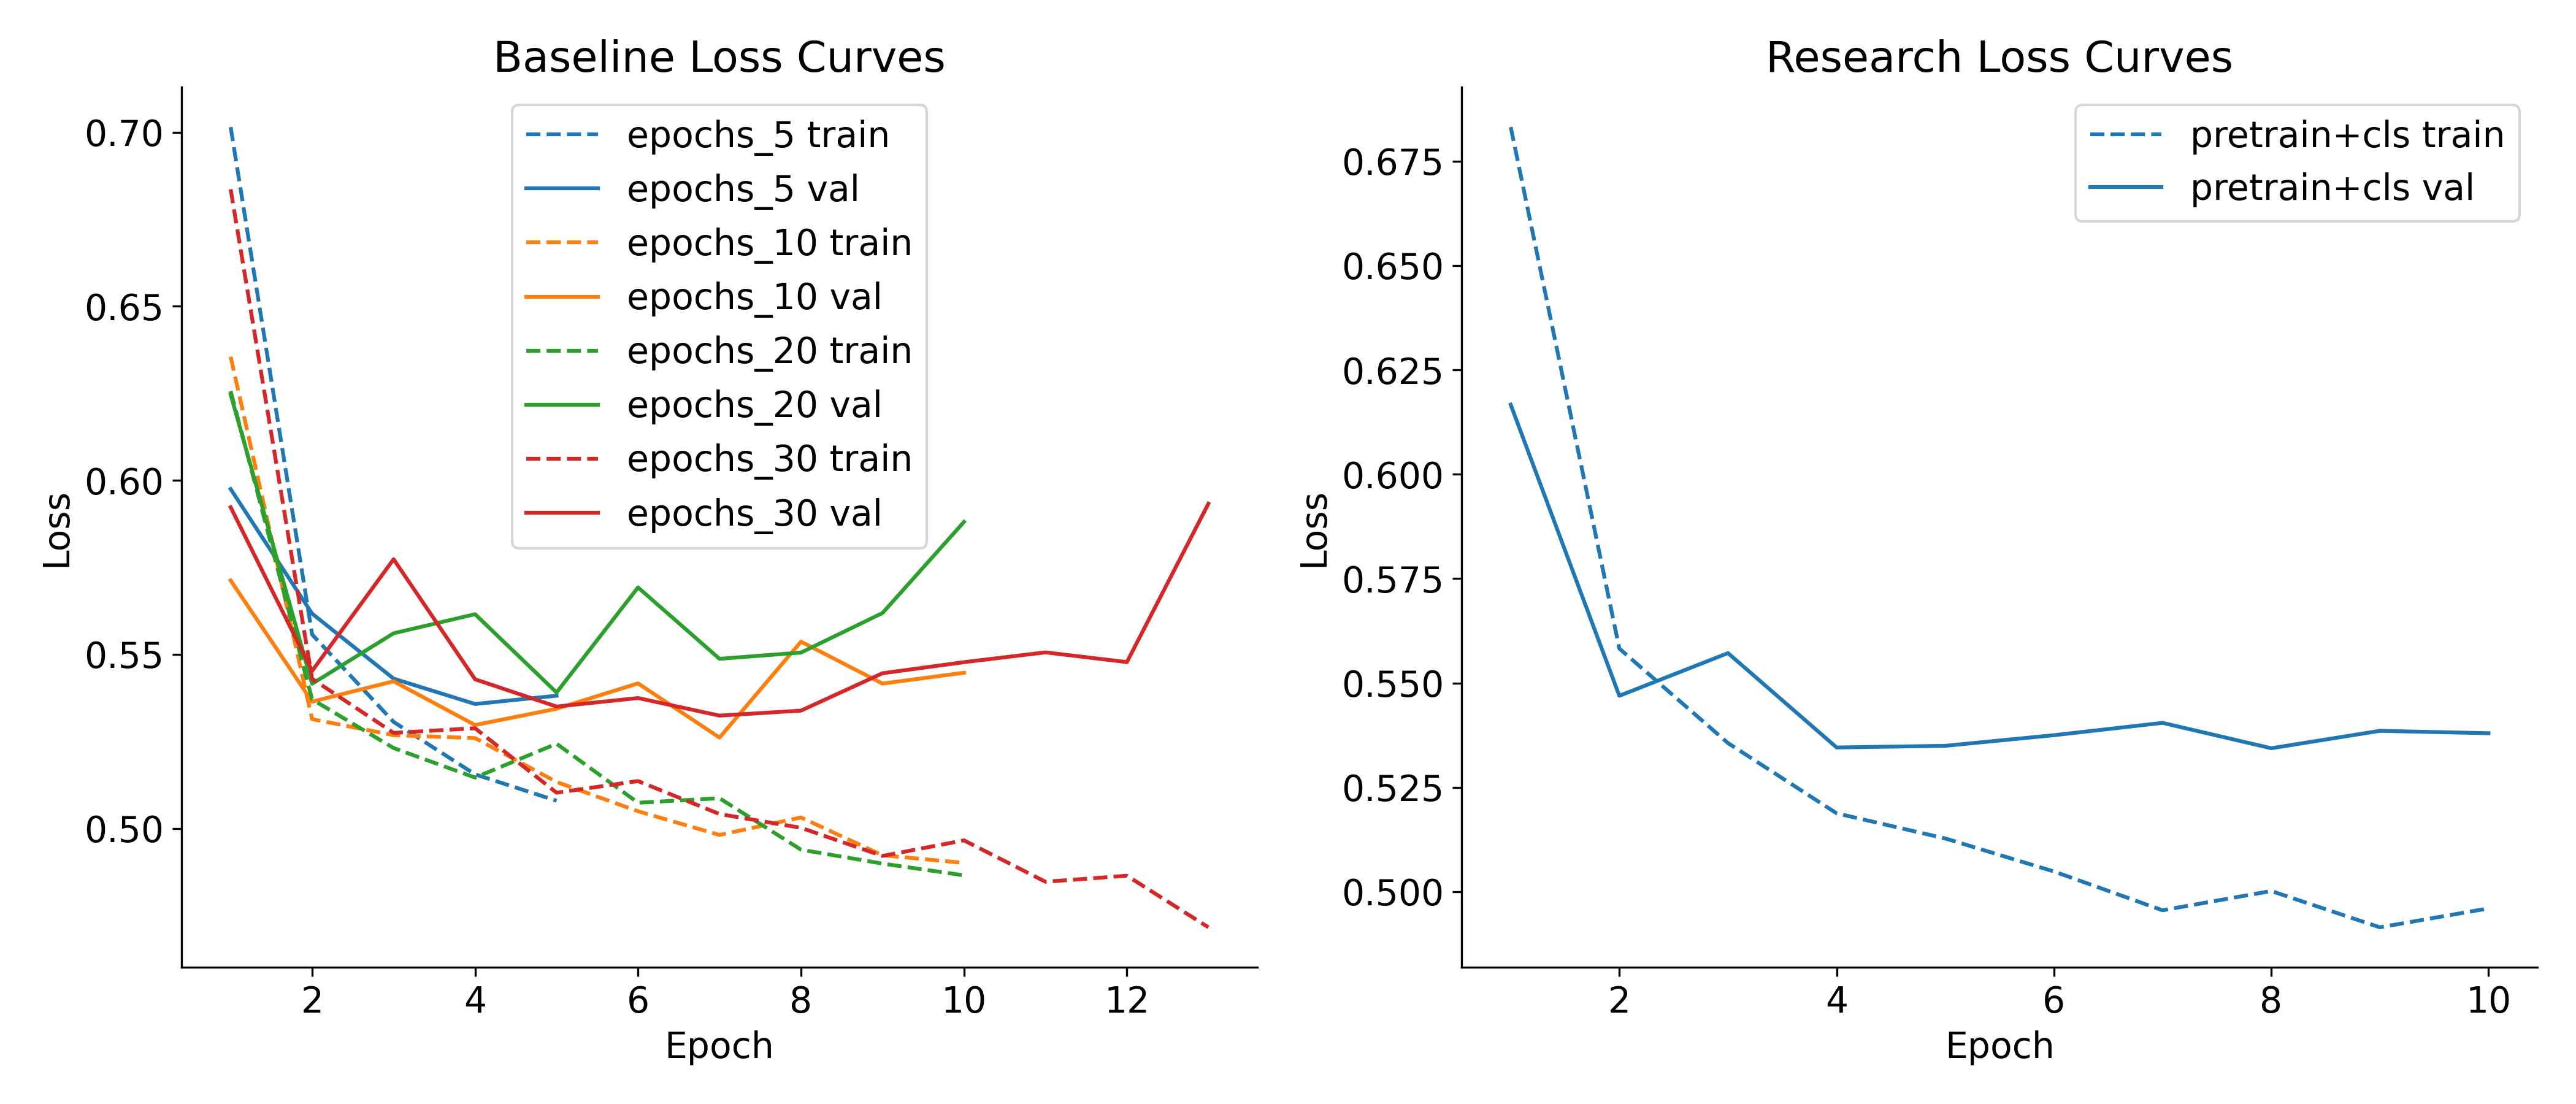
\includegraphics[width=0.7\linewidth]{aggregated_loss_curves.png}
  \caption{Aggregated macro-F1 and loss trends. Both models plateau early, suggesting limited benefit from further training.}
  \label{fig:agg}
\end{figure}

\begin{figure}[t]
  \centering
  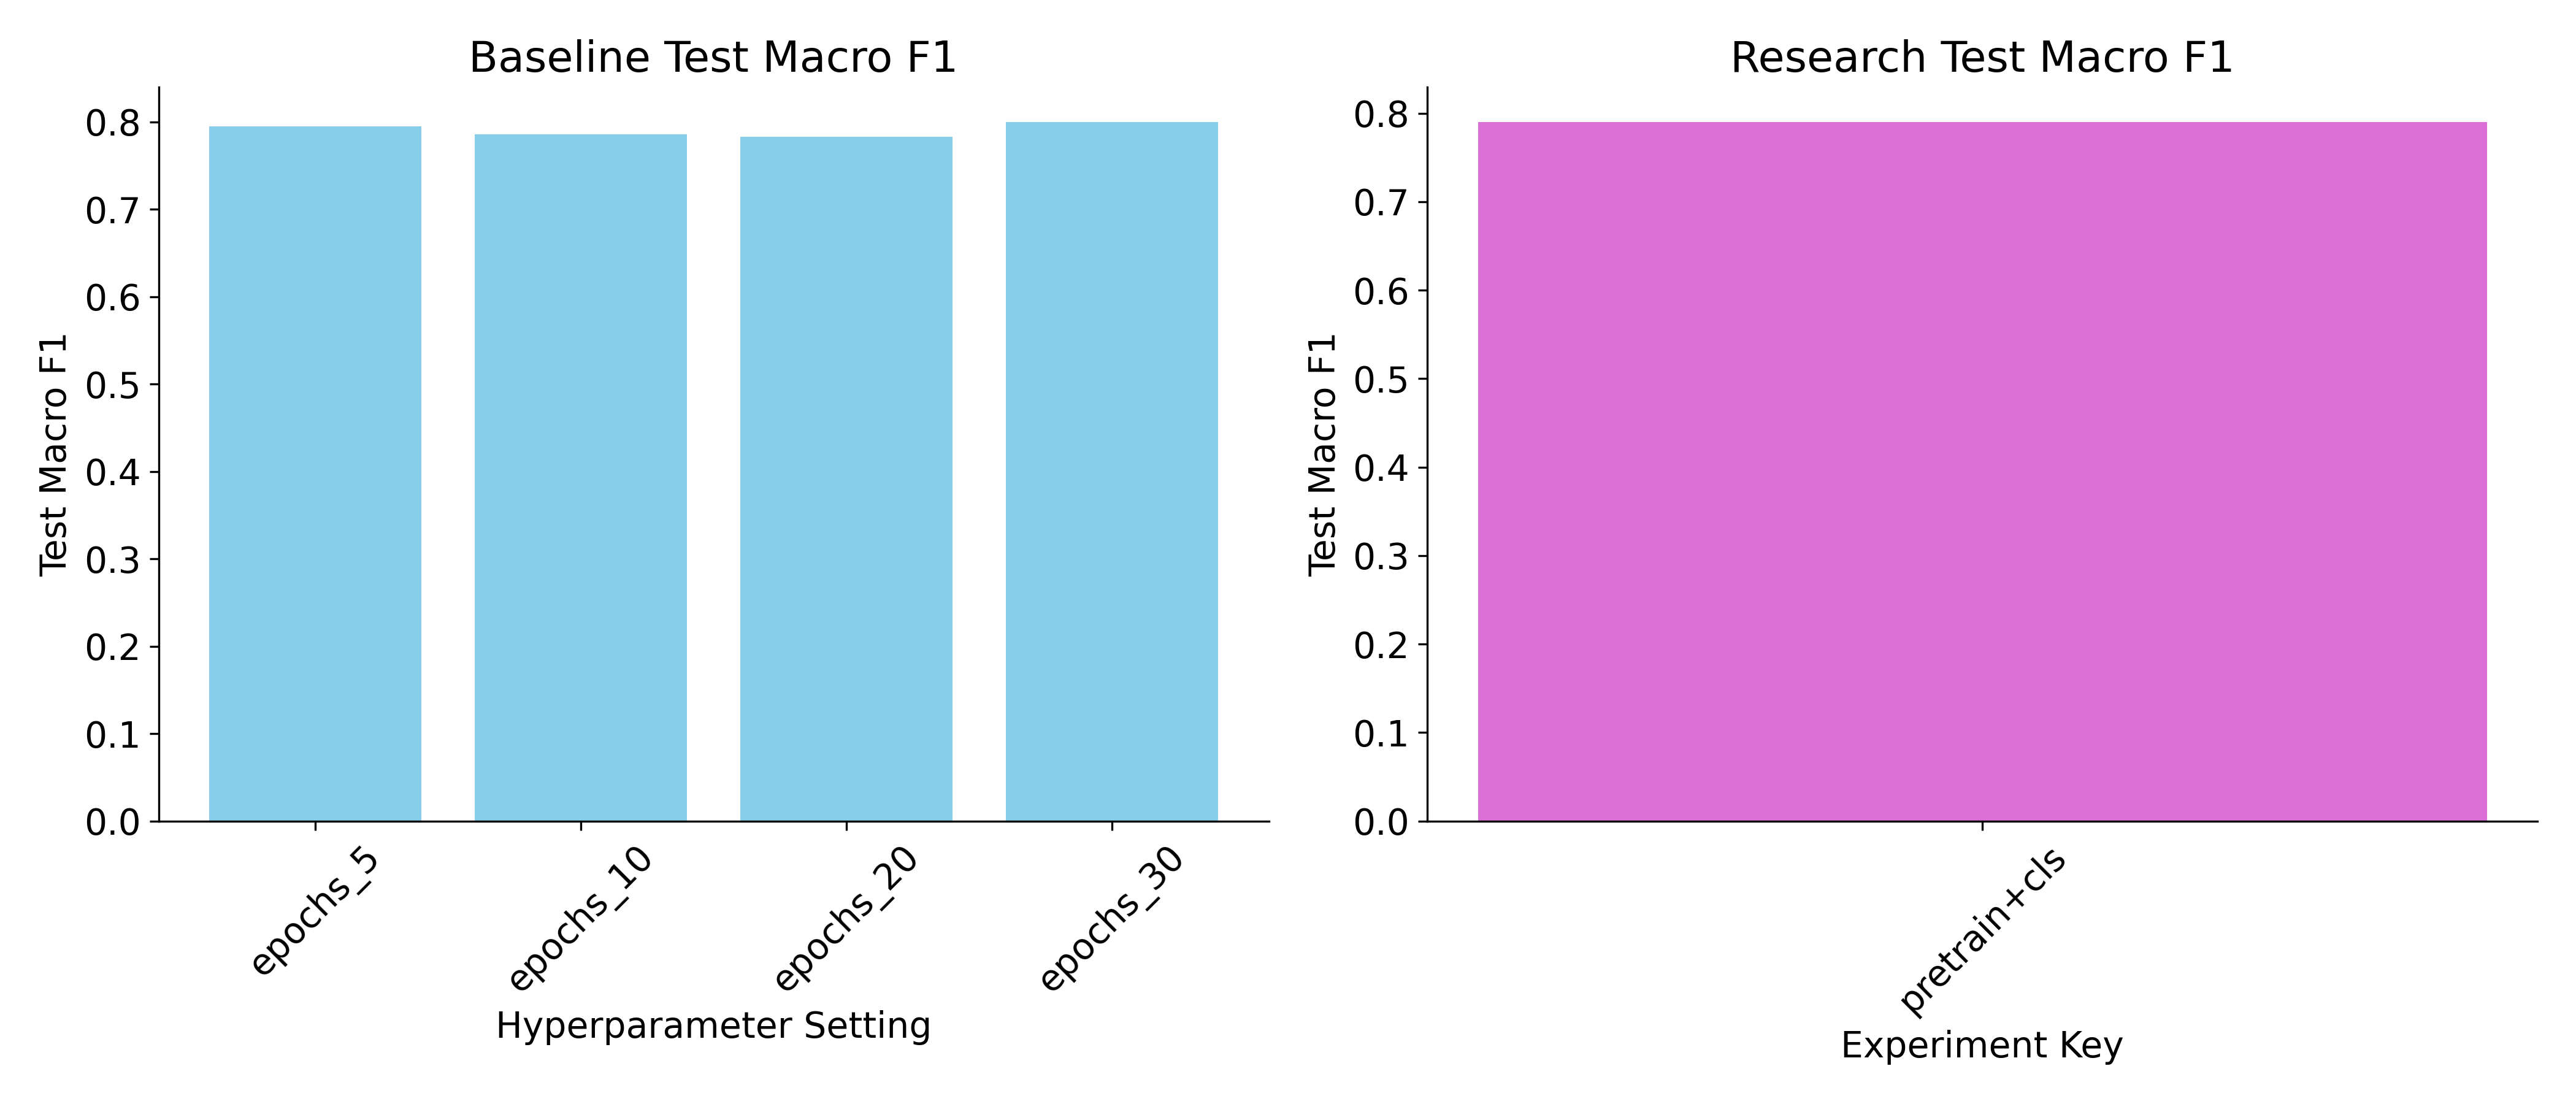
\includegraphics[width=0.6\linewidth]{test_macro_f1_comparison.png}
  \caption{Test macro-F1 comparison between baseline and proposed approach. Gains remain modest.}
  \label{fig:test}
\end{figure}

\section{Conclusion}
We show that popular neural architectures may plateau on symbolic tasks, leaving substantial gaps. Our investigation underscores the need for novel approaches that combine structure-aware methods with standard deep learning. Future work might integrate modular components or data-centric strategies to overcome these limitations.

\bibliography{references}

\clearpage
\appendix

\section{Appendix}
Additional results and hyperparameters are provided here. Supplementary epoch-level comparisons, merged confusion matrices, and per-seed analyses are included for completeness.

\begin{figure}[h!]
  \centering
  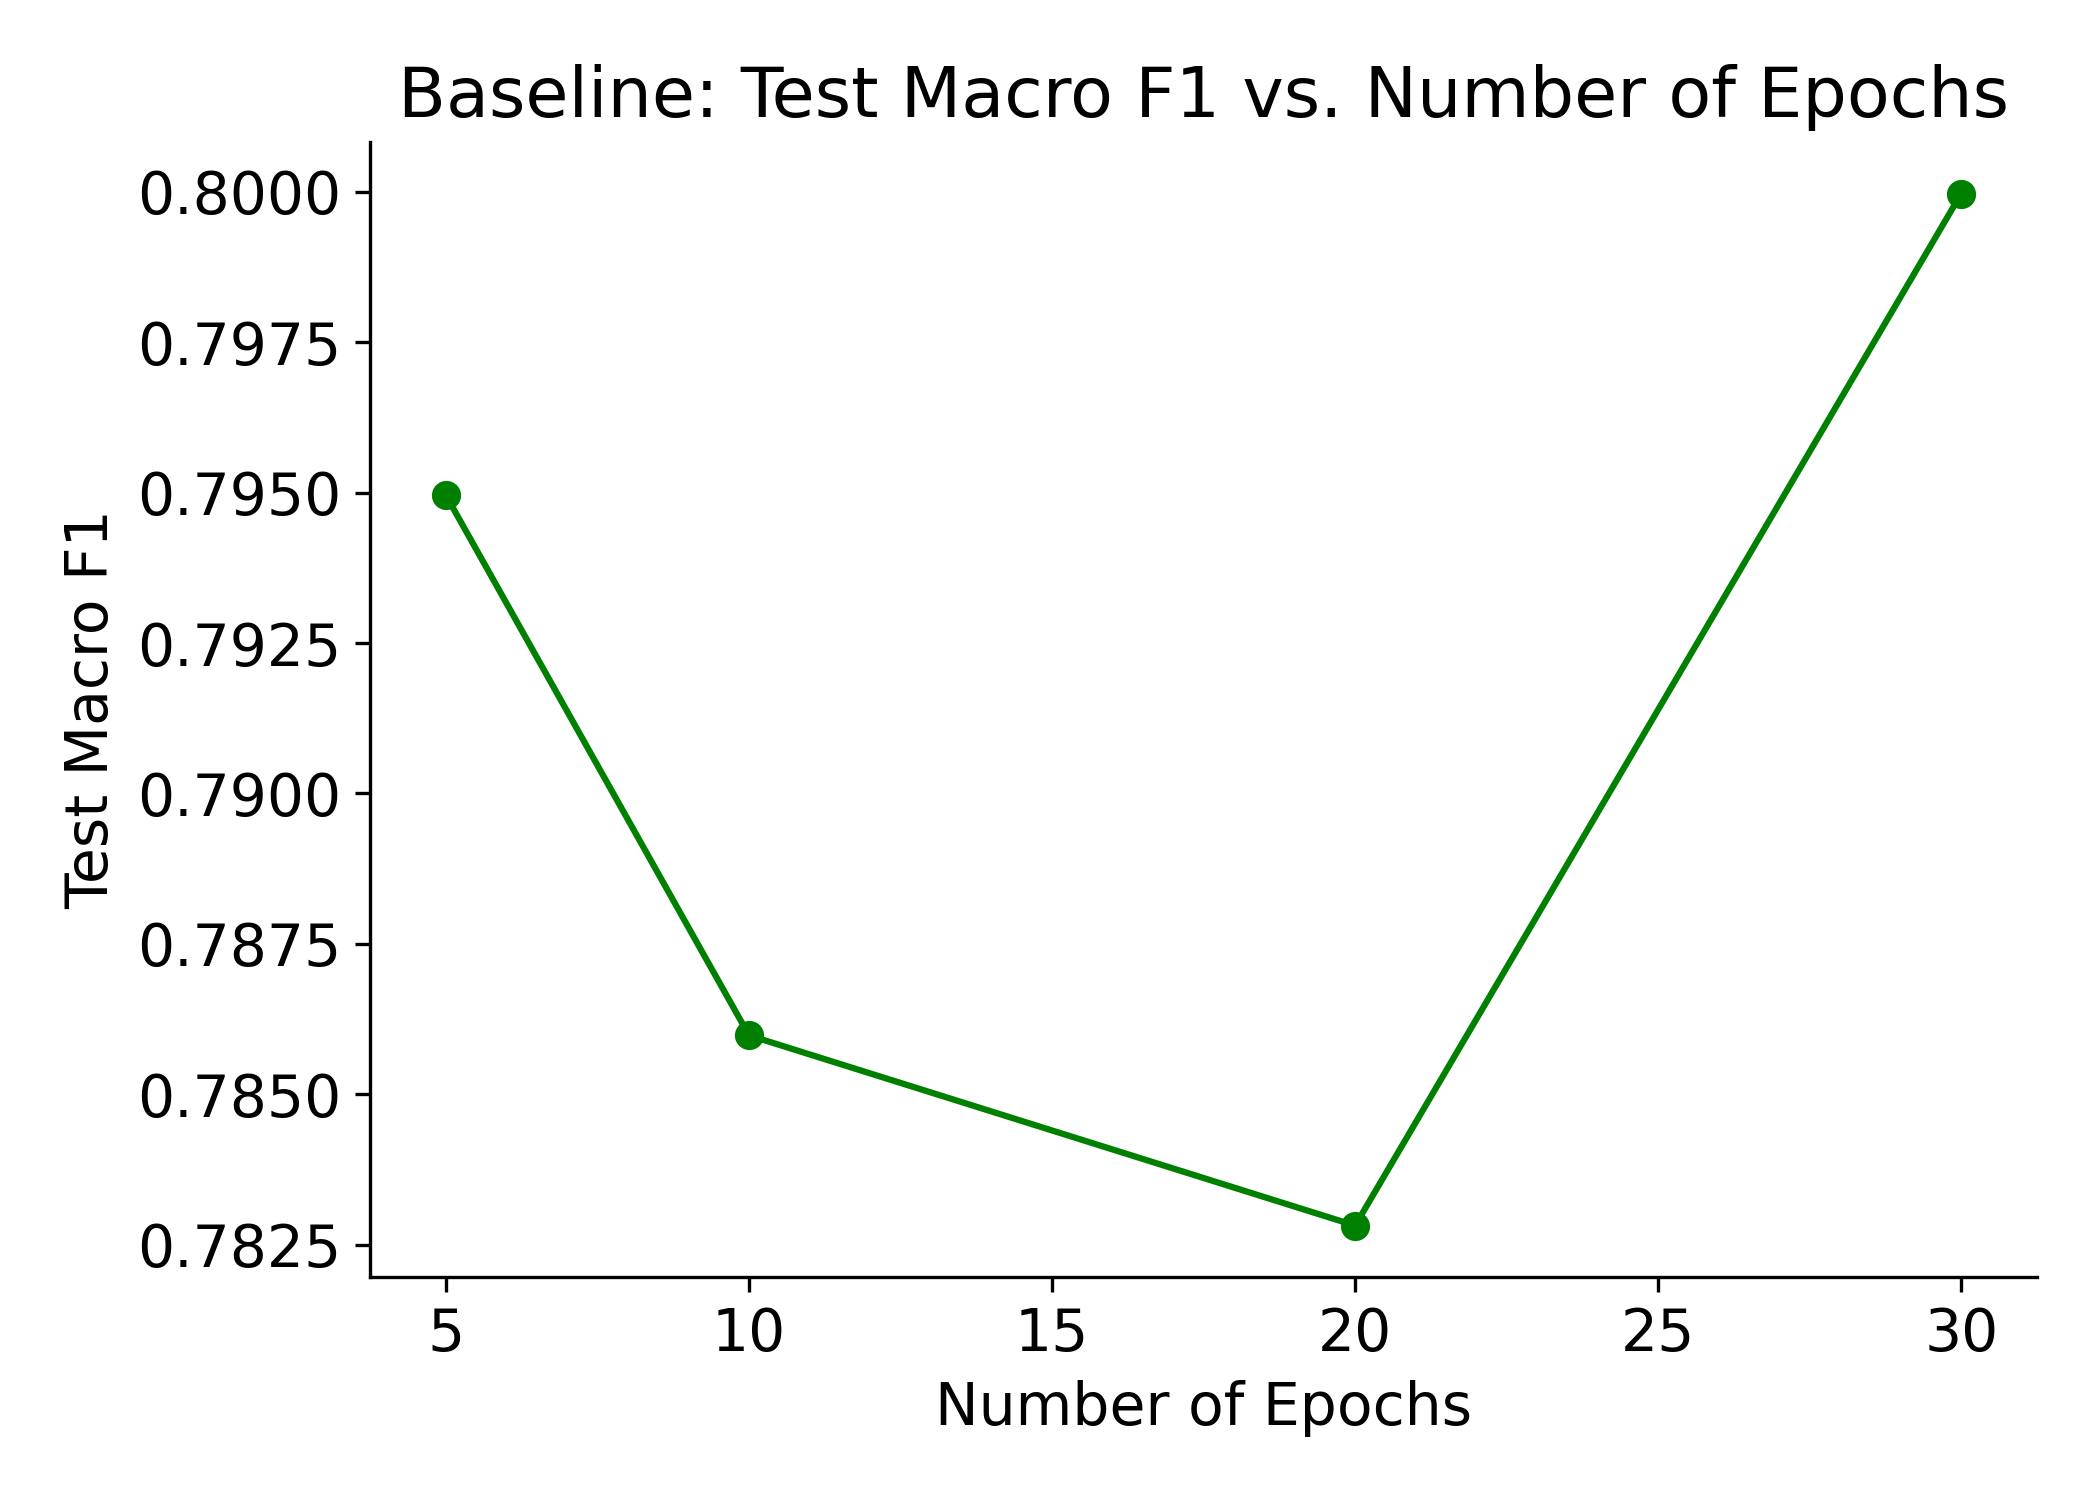
\includegraphics[width=0.6\linewidth]{baseline_test_macro_f1_vs_epochs.png}\\
  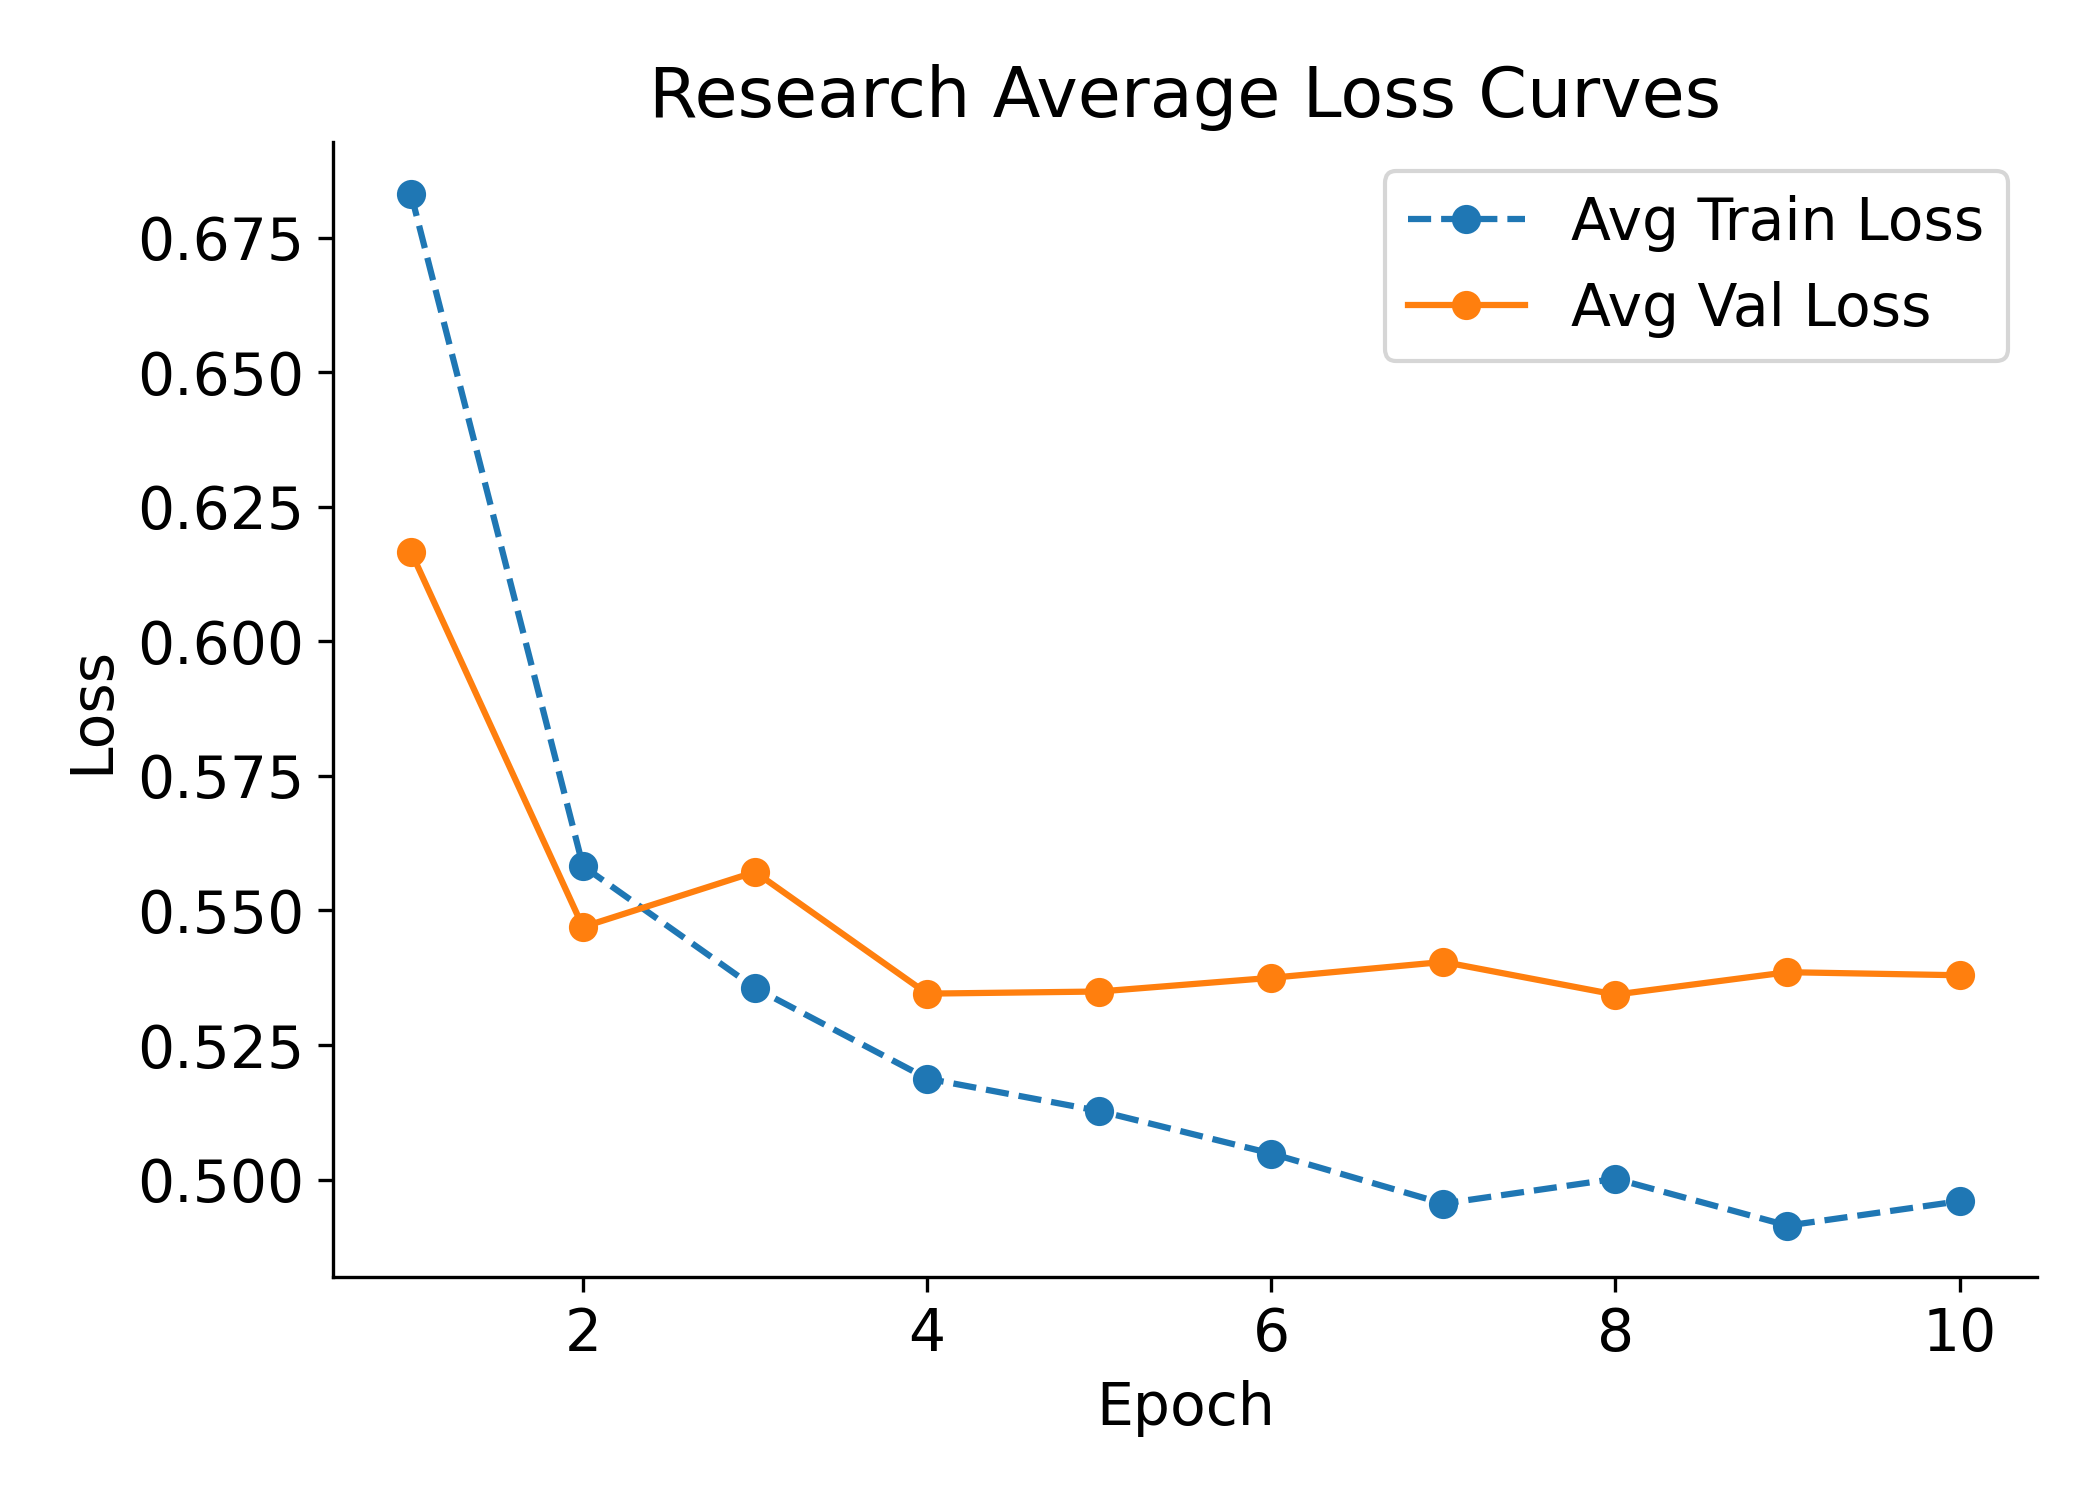
\includegraphics[width=0.65\linewidth]{research_avg_loss.png}\\
  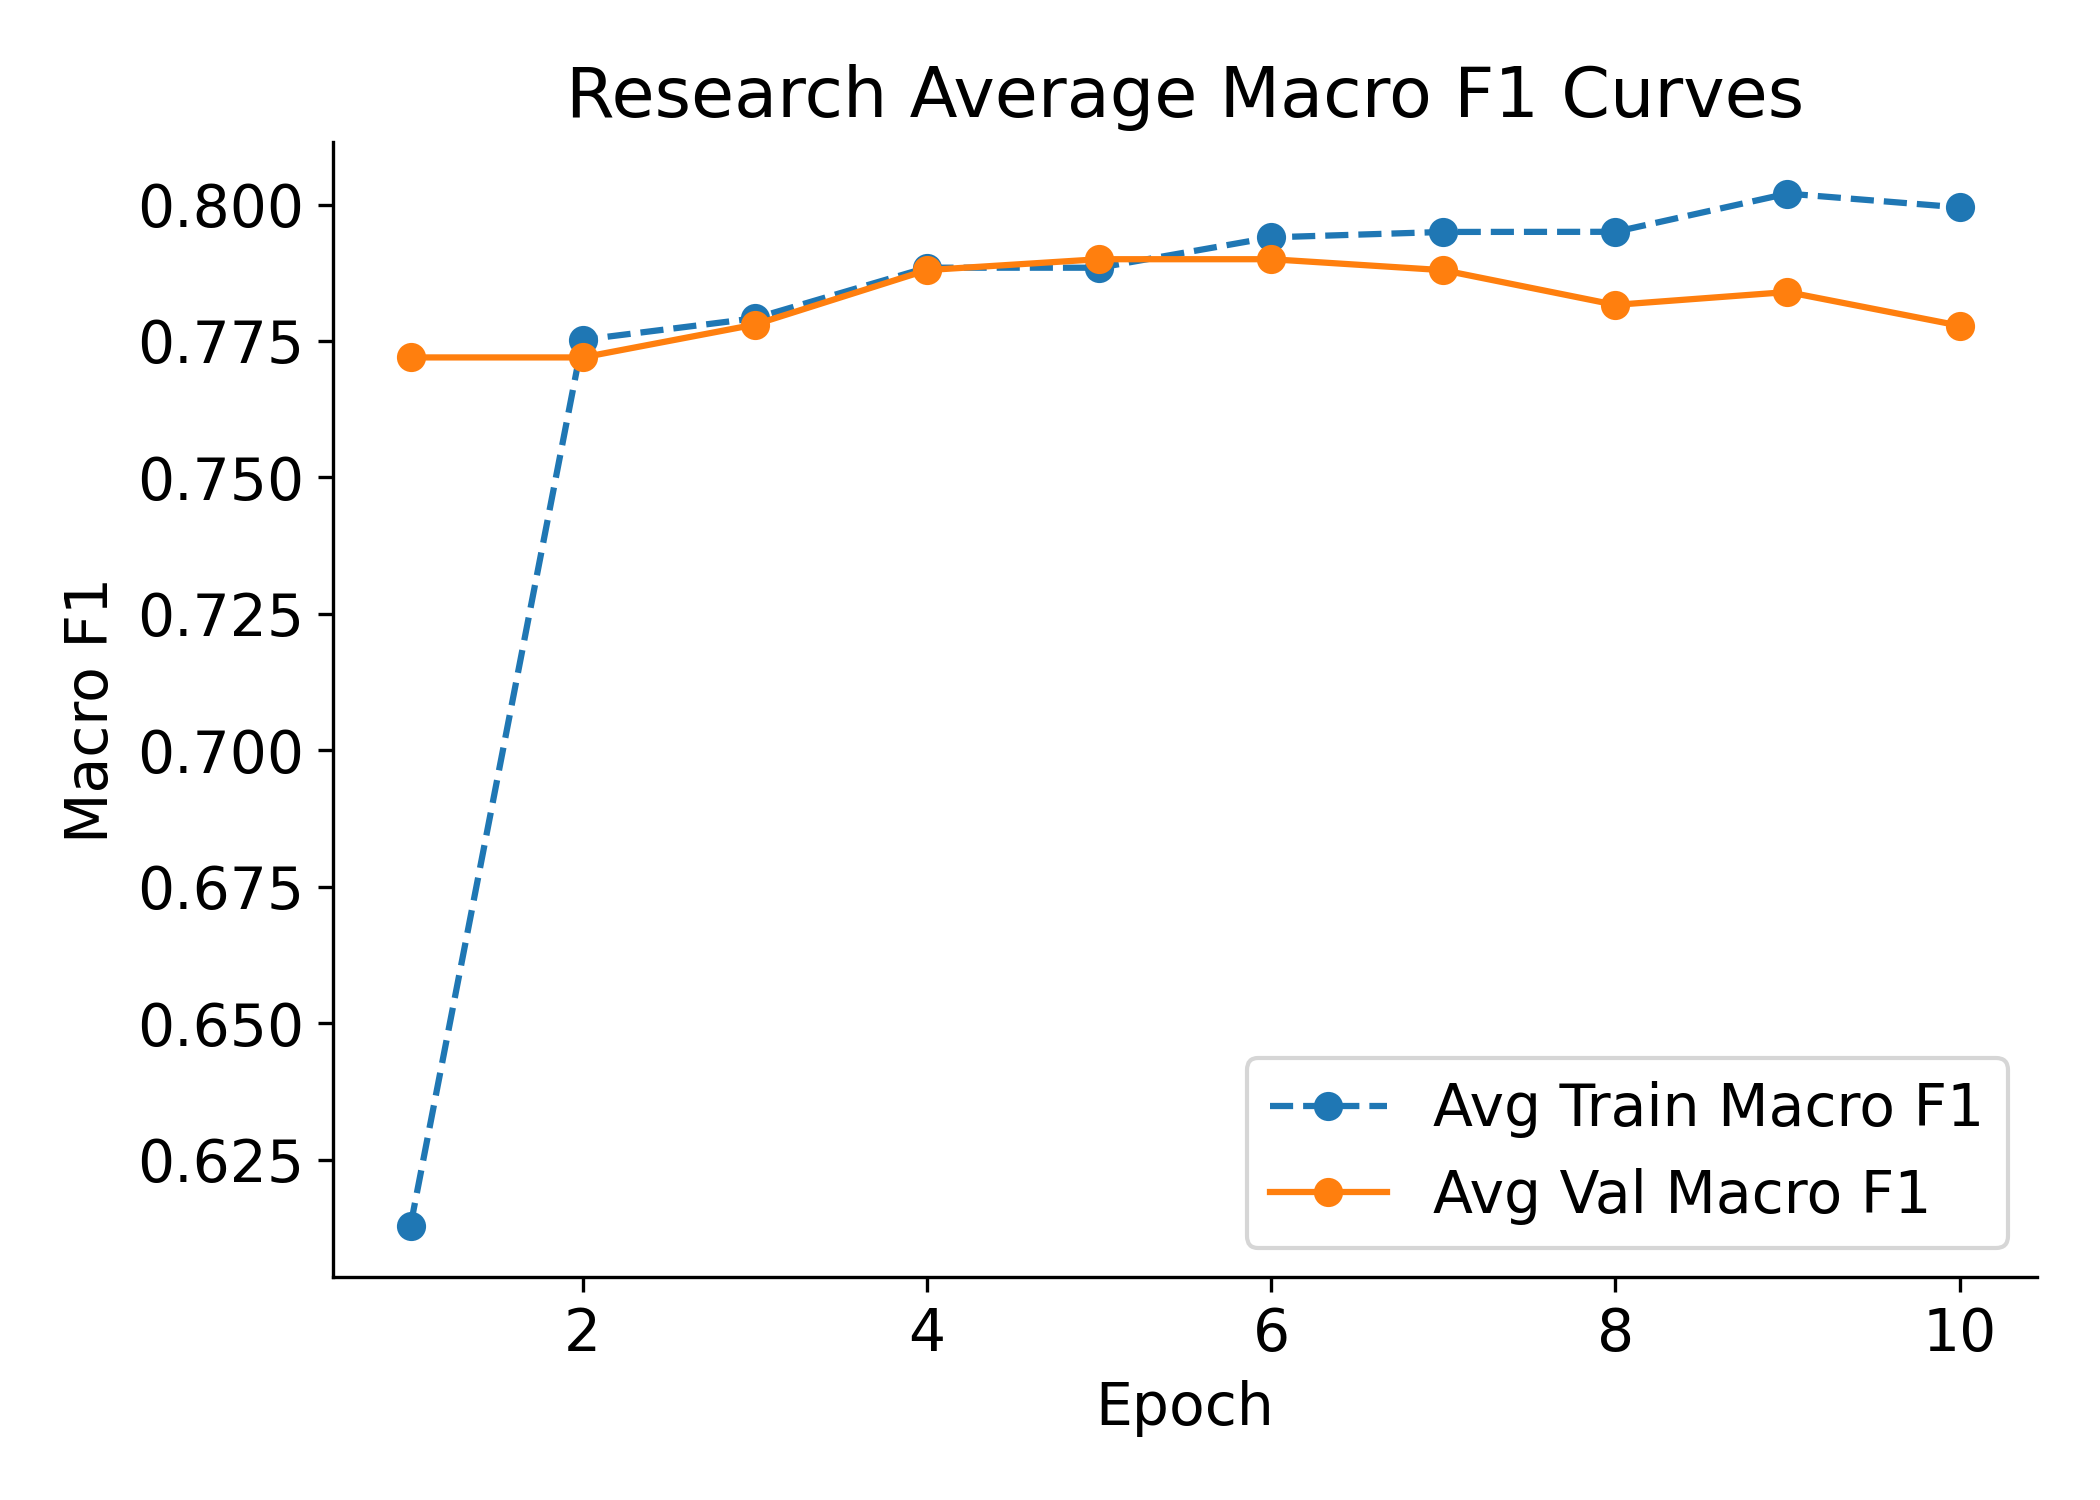
\includegraphics[width=0.65\linewidth]{research_avg_macro_f1.png}
  \caption{Supplementary performance curves and additional aggregated metrics.}
\end{figure}

\begin{figure}[h!]
  \centering
  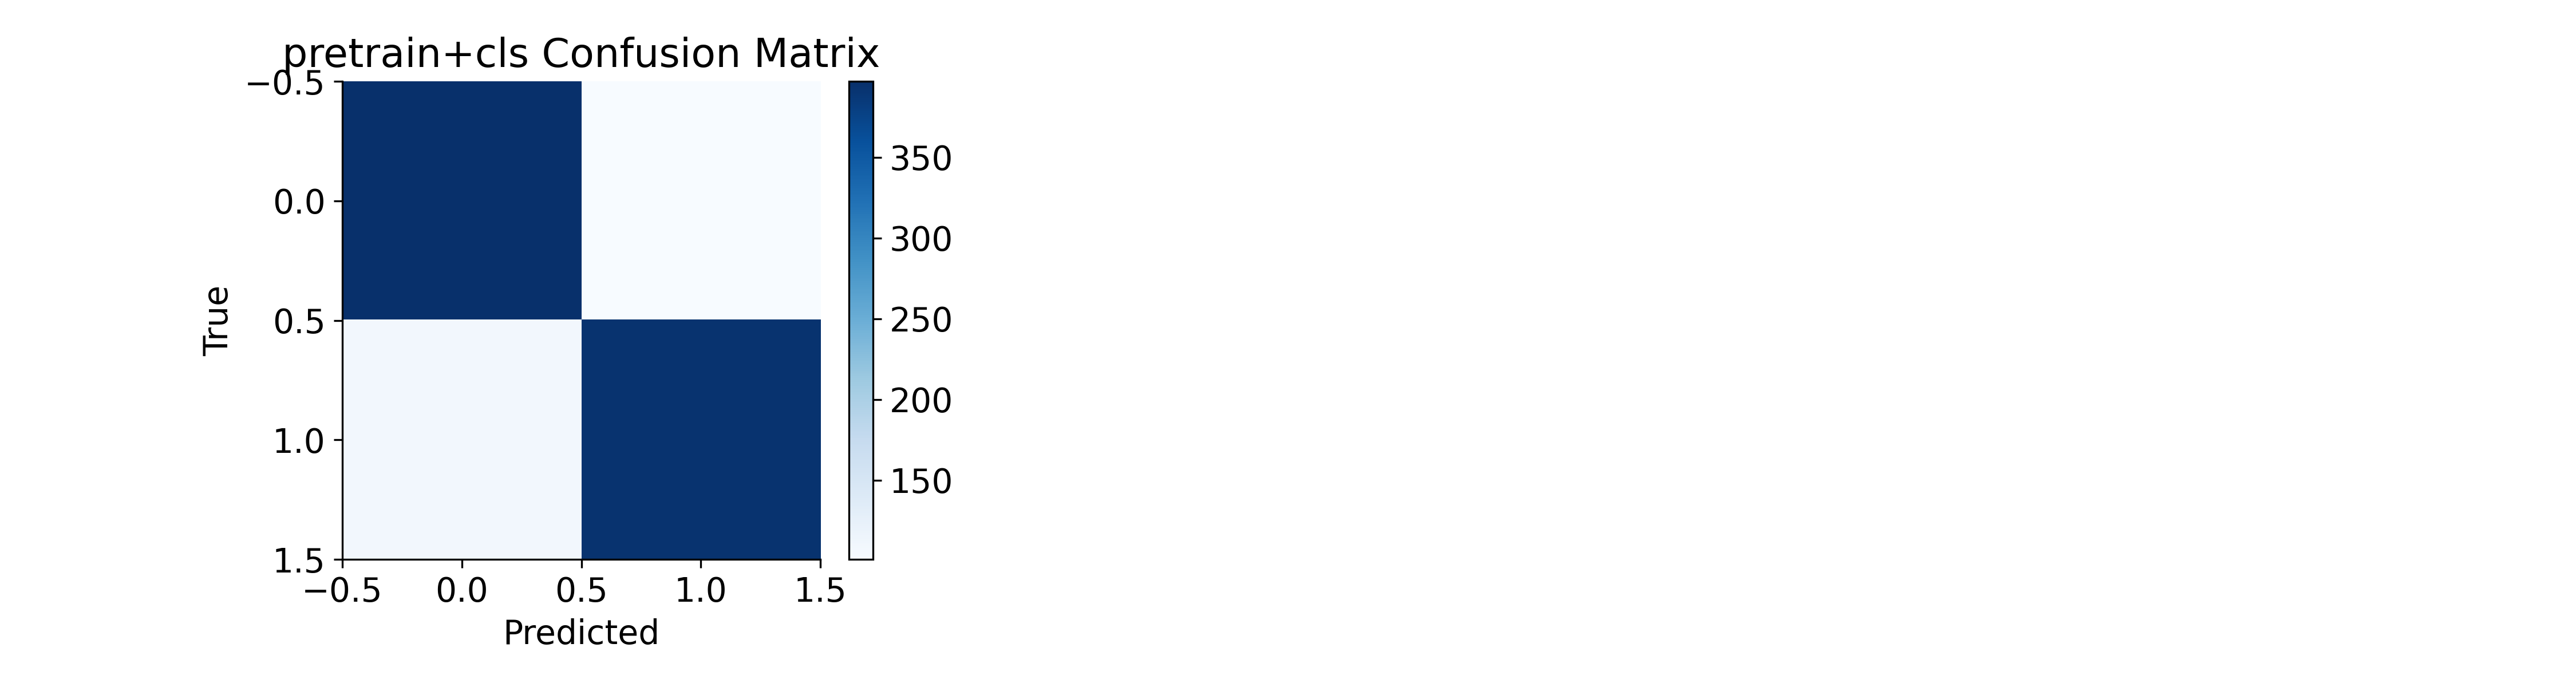
\includegraphics[width=0.95\linewidth]{research_confusion_matrices.png}\\
  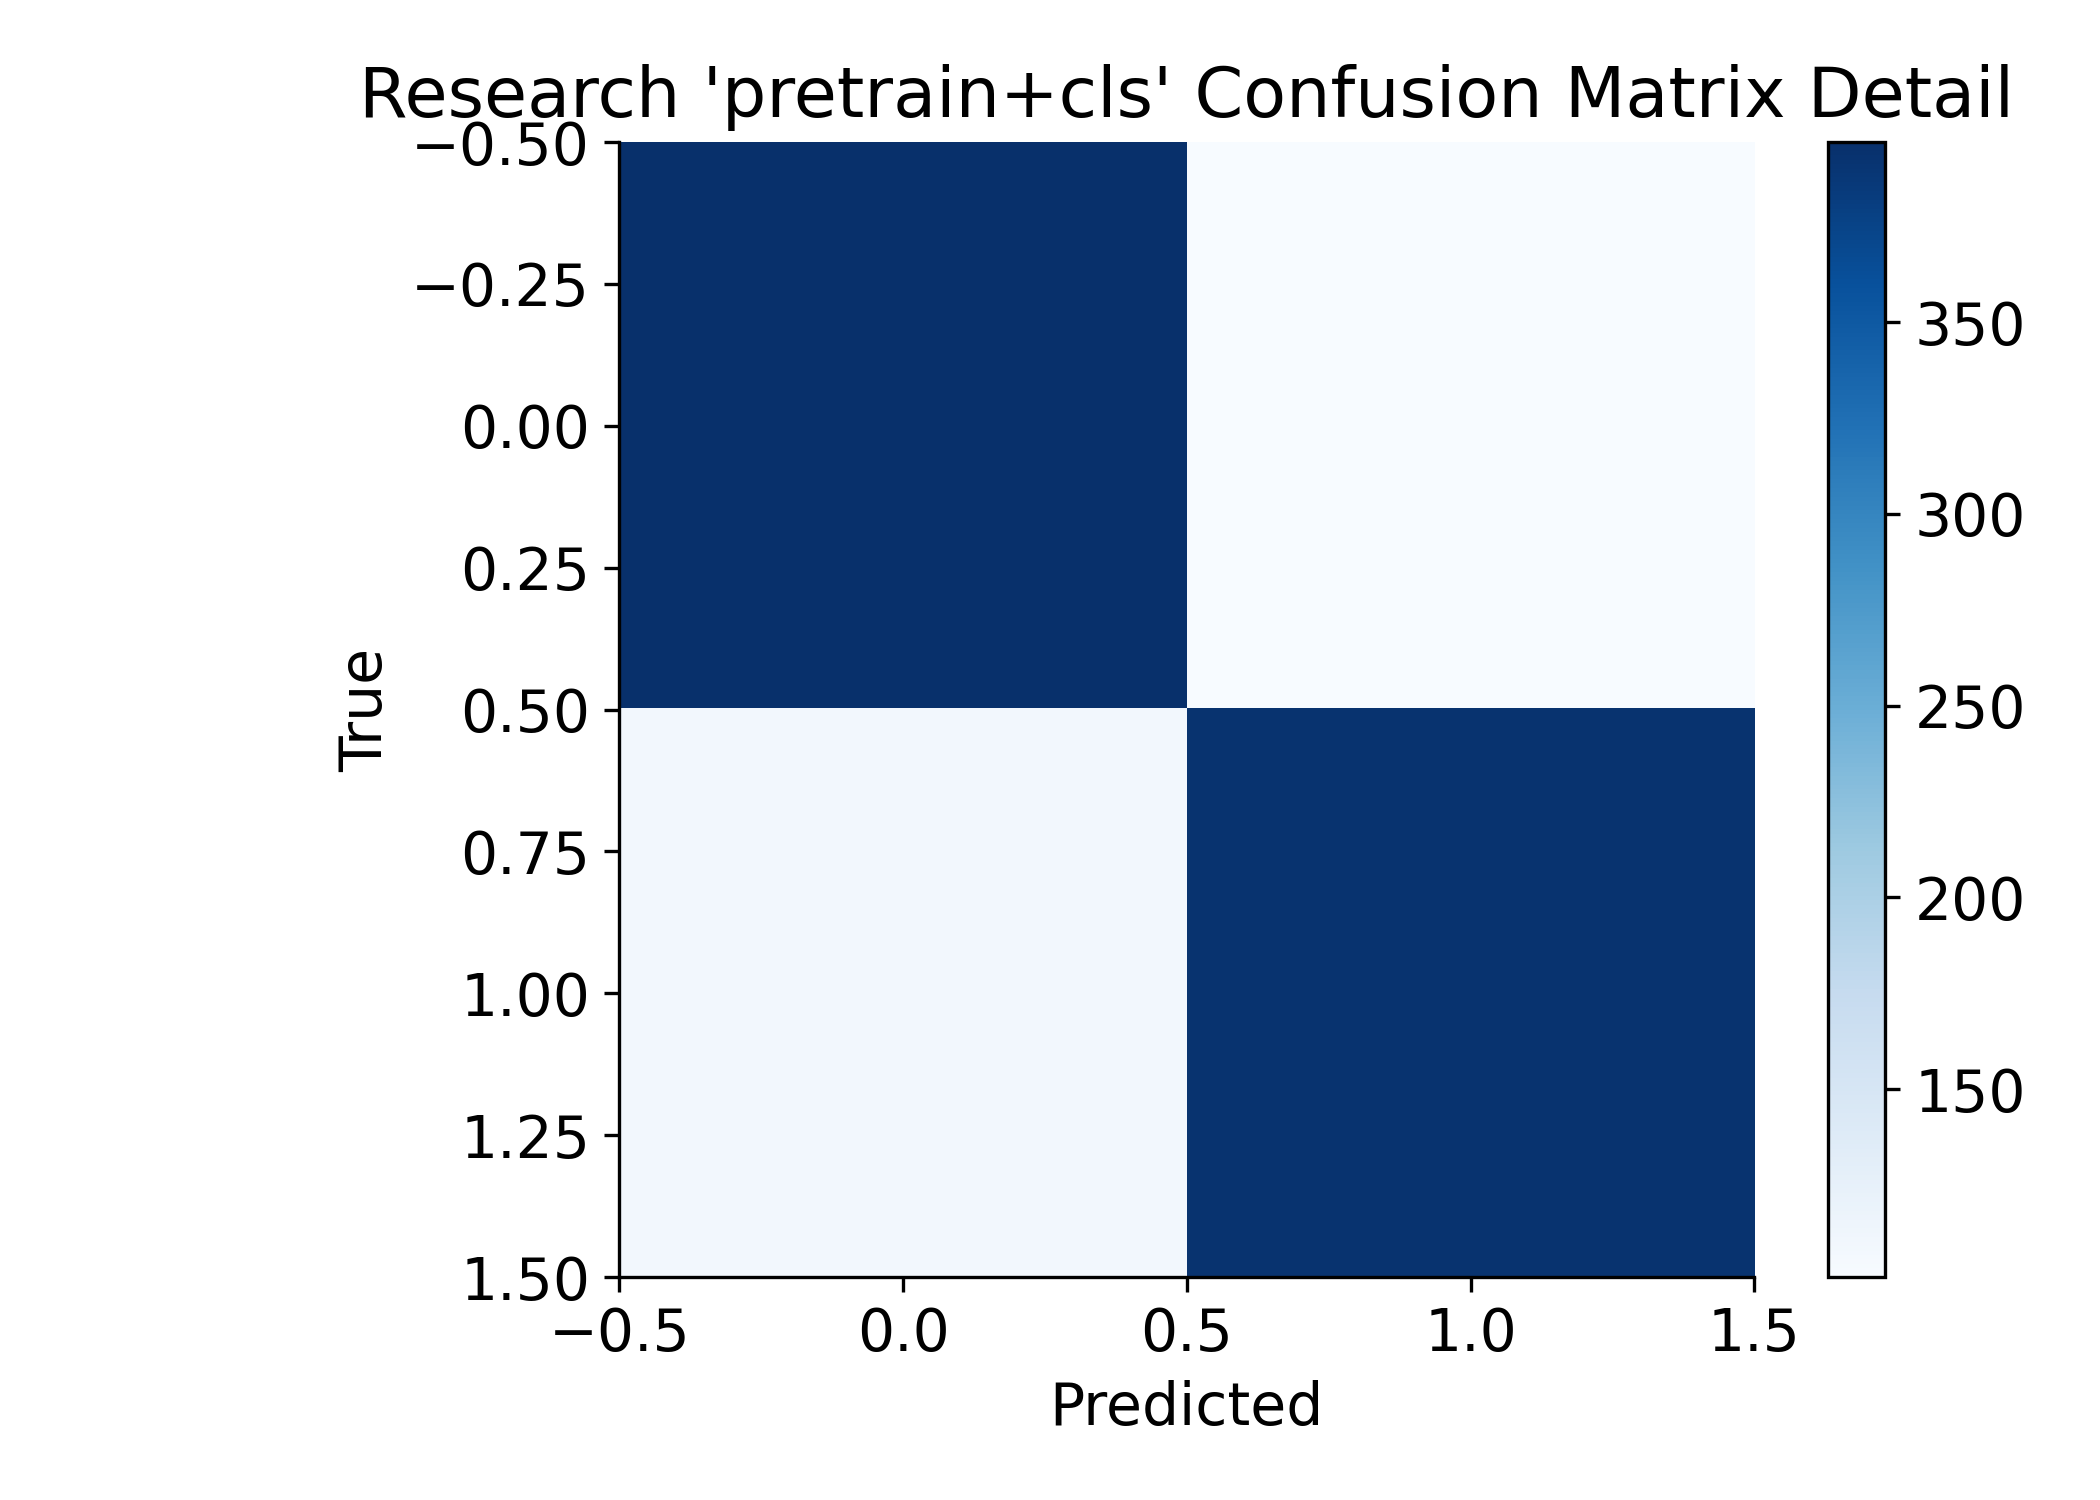
\includegraphics[width=0.95\linewidth]{research_confusion_matrix_detail.png}
  \caption{Combined confusion matrices, capturing both global and class-specific misclassification rates.}
\end{figure}

\end{document}